	\subsection{方針}
	大まかな流れは,次のようである.
	\begin{enumerate}
			\item 分配関数の計算
			\item エネルギー,磁化,磁化率の期待値の計算
			\item 温度,磁場に対する振る舞いを考察
	\end{enumerate}
	この方針は変えず,個々の系に対し様々なテクニックを使う.

	\subsection{すべてのspinが独立にある場合}
	$N$粒子系を考える.
	粒子$j$のspinを$\sigma_j = \pm 1$で指定し,スピン角運動量の固有値は$\pm\mu_0$とする.
	磁場$\mf$中にある系のエネルギー固有値は
	\begin{equation}
			E = -\sum_{j=1}^{N}\mu_0\sigma_j\mf
	\end{equation}
	で,一つの粒子だけに注目したとき
	\begin{align}
			E_j = -\mu_0\sigma_j\mf
	\end{align}
	である.
	spin1つの期待値は期待値の定義から
	\begin{align}
			\expval{\sigma_j} &= \frac{1}{Z_j(\beta)}\qty(\mu_0e^{\beta\mu_0\mf} - \mu_0e^{\beta\mu_0\mf})\\
							  &= \mu_0\tanh(\beta\mu_0\mf)\label{eq:onespin}
	\end{align}
	である.

	独立なので,一粒子の情報がわかれば十分で,一粒子の分配関数は
	\begin{align}
			Z_j(\beta) &= e^{\beta\mu_0\mf} + e^{-\beta\mu_0\mf}\\
				&= 2\cosh(\beta\mu_0\mf)
	\end{align}
	である.よって,$N$粒子あったとき,分配関数は
	\begin{equation}
			Z(\beta) = \qty(2\cosh(\beta\mu_0\mf))
	\end{equation}
	となる.
	エネルギー期待値は
	\begin{align}
			\langle H\rangle &= -\pdv{}{\beta}\log(2\cosh(\beta\mu_0\mf))\\
							 &= -N\mu_0\mf\tanh(\beta\mu_0\mf)
	\end{align}
	である.

	\begin{defn}[磁化]
			磁化を
			\begin{equation}
					m = \frac{1}{N}\sum_{j = 1}^{N}\mu_0\sigma_j
			\end{equation}
			と定める.スピンの平均値と思ってよい.
	\end{defn}
	磁化の期待値は,\eq{eq:onespin}と期待値の線形性から
	\begin{align}
			\expval{m} &= \frac{1}{N}\sum_{j = 1}^{N}\mu_0\expval{\sigma_j}\\
					   &= \mu_0\tanh(\beta\mu_0\mf)
	\end{align}
	である.

	\begin{defn}[$\mf=0$での磁化率]
			磁化率$\chi$を
			\begin{equation}
					\chi = \left.\pdv{m}{\mf}\right|_{\mf=0}
			\end{equation}
			と定める.
			磁場$\mf$を揺すったときの磁石になりやすさと解釈できる.
	\end{defn}

	磁化率も計算する.
	\begin{equation}
			\chi = \frac{\mu_{0}^{2}}{k_{\text{B}}T}\label{eq:single_suscep}
	\end{equation}
	となる.

	本筋とは外れるが,エントロピーを計算する.そのためにまず,Helmholtz free energyの計算をする.
	\begin{align}
			F(\beta, \mf, N)&= -\frac{1}{\beta}\log Z(\beta)\\
							&= -Nk_{\text{B}}T\log\qty(2\cosh\qty(\frac{\mu_0\mf}{k_{\text{B}}T}))
	\end{align}
	ここから,エントロピーが計算できて,
	\begin{align}
			S(\beta, \mf, N) &= -\pdv{}{T}F(\beta, \mf, N)\\
							 &= Nk_{\text{B}}\frac{\mu_0\mf}{k_{\text{B}}T}\qty(\cosh\qty(\frac{\mu_0\mf}{k_{\text{B}}T}) - \log \qty(2\cosh\qty(\frac{\mu_0\mf}{k_{\text{B}}T})))
	\end{align}
	となり,$\mf/k_{\text{B}}$単位で現れる.これを用いて,$(T_1, \mf_1)\rightarrow(T_2, \mf_2)$の断熱準静操作を行うとき,エントロピーが不変なので,この単位も不変である.磁場$\mf$をゆっくり変えることで温度を変えることが\footnote{主に低温を作る.}できる.これを断熱消磁と呼ぶ.

	\subsection{ペアを形成し,ペア同士は独立な場合}
	次に,二つの粒子が相互作用しペアを形成していて,ペア同士は相互作用していない状況を考える.
	粒子数$N$はわかりやすく.偶数としておく.

	このときのエネルギー固有値は
	\begin{equation}
			E_{\sigma} = -J\sum_{j = 1}^{N/2}\sigma_{2j-1}\sigma_{2j} - \mu_0 \mf \sum_{k=1}^{N}\sigma_k\label{eq:exchange}
	\end{equation}
	とする.第一項が相互作用による項でHeisenberg交換相互作用とよばれる.

	$J$は物質による定数で,$J$が正の場合ペアのスピンは揃いやすく,負の場合,反対を向きやすい.

	以上の設定で考える.

	まず,ペアたちは独立なので,$(\sigma_1, \sigma_2)$だけ選んで考える.
	\eq{eq:exchange}にでてくる量を計算し,Table \ref{tab:exchange_interaction}にまとめておく.
	\begin{table}[tbp]
			\centering
			\caption{\eq{eq:exchange}のスピンを含む箇所の計算結果.}
			\begin{tabular}{c|cccc}\hline
					$(\sigma_1, \sigma_2)$ & $(1, 1)$ & $(1, -1)$ & $(-1, 1)$ & $(-1, -1)$\\\hline
					$\sigma_1\sigma_2$ & $1$ & $-1$ & $-1$ & $1$\\
					$\sigma_1 + \sigma_2$ & $2$ & $0$ & $0$ & $-2$\\
					$E_{N=2}$ & $-J-2\mu_0\mf$ & $J$ & $J$ & $-J+2\mu_0\mf$\\\hline
			\end{tabular}
			\label{tab:exchange_interaction}
	\end{table}

	これで,分配関数が計算できる.

	\begin{align}
			Z(\beta) &= e^{-\beta(-J - 2\mu_0\mf)} + 2e^{-\beta J} + e^{-\beta(-J+2\mu_0\mf)}\\
					 &= 2e^{\beta J}\qty(\cosh(2\beta\mu_0 \mf) + e^{-2\beta J}).
	\end{align}

	エネルギー期待値は
	\begin{align}
			\langle H \rangle &= -\pdv{}{\beta}\log Z(\beta)\\
							  &= -\frac{N}{2}\frac{J(e^{-2\beta J} - \cosh(2\beta\mu_0\mf)) - 2\mu_0\mf\sinh(2\beta\mu_0 \mf)}{\cosh(2\beta\mu_0\mf) + e^{-2\beta J}}
	\end{align}
	となる.ここで,$\mf = 0$とすると,
	\begin{equation}
			\langle H \rangle = -\frac{N}{2}\tanh\beta J
	\end{equation}
	である.

	spinのペアの期待値は
	\begin{align}
			\langle \sigma_1 + \sigma_2\rangle &= \frac{1}{Z(\beta)}\qty(2e^{\beta(J + 2\mu_0\mf)} - e^{-\beta(J-2\mu_0\mf)})\\
										&= \frac{2\sinh(2\beta \mu_0 \mf)}{\cosh(2\beta\mu_0 /mf) + e^{-2\beta J}}
	\end{align}
	磁化は
	\begin{align}
			\langle m \rangle &= \left\langle \frac{1}{N}\sum_{j = 1}^{N}\sigma_j\right\rangle\\
							  &= \frac{1}{N}\sum_{j = 1}^{N/2}\langle \sigma_{2j-1}\sigma_{2j}\rangle\\
							  &= \frac{\sinh(2\beta\mu_0\mf)}{\cosh(2\beta\mu_0\mf) + e^{-2\beta J}}\\
							  &= \frac{2\beta\mu_0^2\mf + \O\qty((\beta\mu_0\mf)^3)}{1 + \O\qty((\beta\mu_0\mf)^2) + e^{-2\beta\mu_0\mf}}
	\end{align}
	となる.最後は磁化率を求めるために$\mf$を含む冪で展開した.

	磁化率は$\mf$で微分して$\mf = 0$とするので,二次以上の項は消えて,
	\begin{align}
			\chi(\beta) &= \left.\pdv{\expval{m}}{\mf}\right|_{\mf=0}\\
					 &= \frac{2\beta\mu_0^2}{1 + e^{2\beta J}}
	\end{align}
	となる.

	\subsection{1-d Ising model}
	エネルギー固有値は
	\begin{equation}
			E_{\sigma} = -J\sum_{\langle i, j \rangle} \sigma_i\sigma_j - \mu_0\mf \sum_{i=1}^{N}\sigma_i
	\end{equation}
	とする.ここで,$\langle i, j\rangle$は隣り合う$i$, $j$に関して和をとることを表し,周期的境界条件$\sigma_{N+1} = \sigma_1$を入れると,
	\begin{equation}
			E_{\sigma} = -J\sum_{i = 1}^{N}\sigma_{i}\sigma_{i+1} - \mu_0\mf\sum_{i=1}^{N}\qty(\frac{\sigma_i+\sigma_{i+1}}{2})
	\end{equation}
	と書き換えることができる.

	分配関数は
	\begin{align}
			Z(\beta) &=\sum_{\sigma} e^{E_{\sigma}}\\
			 &= \sum_{\sigma}e^{\sum_{i=1}^{N}\qty(\beta J\sigma_i\sigma_j + \beta \mu_0\mf (\sigma_i + \sigma_{i+1})/2)}\\
			 &= \sum_{\sigma_1 = \pm 1}\cdots\sum_{\sigma_N=\pm 1}\prod_{i=1}^{N}e^{\beta J\sigma_i\sigma_j + \beta \mu_0\mf (\sigma_i + \sigma_{i+1})/2}\\
			 &= \sum_{\sigma_1 = \pm 1}\cdots\sum_{\sigma_N=\pm 1}\prod_{i=1}^{N}M_{\sigma_i, \sigma_{i+1}}
	\end{align}
	となる.行列$M$は転送行列とよばれ,
	\begin{equation}
			M = \begin{pmatrix}
					e^{\beta J + \beta\mu_0\mf} & e^{-\beta J}\\
					e^{-\beta_j} & e^{\beta J - \beta \mu_0\mf}
			\end{pmatrix}
	\end{equation}
	である.さらに分配関数は計算できて,
	\begin{align}
			Z(\beta) &= \Tr\qty(M^N)\\
					 &= \lambda_{+}^{N} + \lambda_{-}^{N}
	\end{align}
	で,$\lambda_{\pm}$は転送行列の固有値で
	\begin{equation}
			\lambda_{\pm} = e^{\beta J}\cosh\beta\mu_0\mf \pm \sqrt{e^{2\beta J}\cosh^2\beta\mu_0\mf - 2\sinh\beta J}
	\end{equation}
	である.

	これを用いて,各物理量を求める.
	自由エネルギー密度は
	\begin{align}
			f_N(\beta) &= -\frac{1}{\beta N}\log Z(\beta)\\
					   &= -\frac{1}{\beta}\log\lambda_{+} - \frac{1}{\beta N}\log\qty(1 + \frac{\lambda_{-}}{\lambda_{+}})
	\end{align}
	なので,$N\to \infty$で$f(\beta ) = -\log\lambda_{+}/\beta$となる.

	磁化は
	\begin{equation}
			m(\beta, \mf) = \frac{\mu_0\sinh\beta\mu_0\mf}{\sqrt{\sinh^2\beta\mu_0\mf + e^{-4\beta J}}}
	\end{equation}
	で,磁化率は
	\begin{equation}
			\chi(\beta) = \beta \mu_0^2e^{2\beta J}
	\end{equation}
	である.

	これらは連続関数で1-d Ising modelは相転移を起こさないこと\footnote{強いていえば,$\beta\to\infty$で発散するので,絶対零度が相転移点ということもできる. }がわかる.

	\subsection{2-d Ising model}
	二次元では相転移を起こす.しかし,直接解くのは大変である\footnote{2022/04/19時点では私は解けていない.}.

	他の状況でも使える,かなり雑だが有用な近似である平均場近似の方法と相転移温度を正しく導出できるKramers--Wannier双対性を用いた議論\footnote{元ネタは2020年度現代物理学第9回.\url{https://member.ipmu.jp/yuji.tachikawa/lectures/2020-komaba/}}を行うことにする.


	\subsubsection{平均場近似}
	
	$d$次元のIsing模型を考える.
	任意に格子点を選び,その上のスピン変数を$\sigma_0$と呼ぶことにする.
	このスピンの最近接の点は$2d$個ある.これらを$\sigma_i,\ i=1,\ldots,2d$と呼び,$\sigma_0$に着目したエネルギーを考えると
	\begin{equation}
			E_{\sigma_0} = \qty(-J\sum_{i=1}^{2d}\sigma_i -\mu_0\mf)\sigma_0
	\end{equation}
	である.ここで,$\sum_{i=1}^{2d}\sigma_i \to 2d\psi$と置き換える.$\psi = \sum_{i=1}^{2d}\sigma_i/(2d)$でスピンの期待値である.ゆらぎのある確率変数を定数で置き換えたもので,これが平均場近似の第一ステップである.


	この分配関数は
	\begin{equation}
			Z_{\sigma_0}(\beta) = 2\cosh(2d\beta J\psi + \beta\mu_0\mf)
	\end{equation}
	であり,$\sigma_0$の期待値は
	\begin{equation}
			\langle\sigma_0\rangle = \tanh(2d\beta J \psi + \beta \mu_0\mf)
	\end{equation}
	である.
	ところが,$\sigma_0$は任意に取ったので,期待値は$\langle \sigma_0 \rangle = \psi$のように思える.これが平均場近似の第二ステップである.

	結局,平均場近似では
	\begin{equation}
			\psi = \tanh(2d\beta J \psi)
	\end{equation}
	を$\psi$について解くことに帰着する.このような方程式をbootstrap方程式\footnote{self-consistent方程式というほうが多い気もするが,bootstrapのほうがおしゃれで好き.沼に落ちたとき自分で自分の靴紐を引っ張って脱出することが語原らしい.}という.

	特に,$\mf = 0$, $d = 2$の状況を考える.
	bootstrap方程式は
	\begin{equation}
			\psi = \tanh(4\beta J \psi)\label{fig:2d-bootstrap}
	\end{equation}
	である.
	\begin{figure}
			\centering
			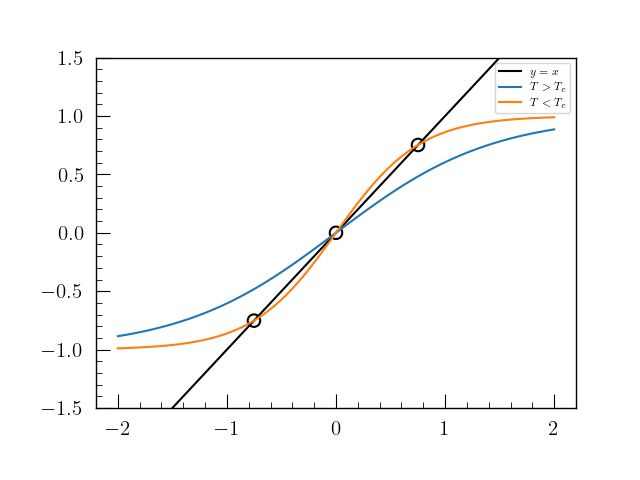
\includegraphics[width=10cm]{./doc/src/img/mean_field.png}
			\caption{bootstrap方程式\eqref{fig:2d-bootstrap}の左辺と右辺の概形.白丸が解で,パラメータ$\beta$によって解の振る舞いが変わることがわかる.対称性があるにもかかわらず,低温領域では$\psi=0$ではない部分にnon trivialな解をもつ.このような状況をSSB(Spontaneous Symmetry Breaking)という.}
	\end{figure}
	この解はFigure \ref{fig:2d-bootstrap}のようにパラメータ$\beta$によって振る舞いがかわり,$\tanh$の原点での傾き$ 4\beta_{\text{mf}} J = 1$が分岐点になっている.
	すなわち,平均場近似での臨界点は
	\begin{equation}
			\beta_{\text{mf}} J= \frac{1}{4} = 0.25
	\end{equation}
	であり,後述する正しい値(Eq. \eqref{Tc_2d-Ising})とは異なる.

	\subsubsection{Kramers--Wannier双対性}
	
	ここでは見やすさの都合上,分配関数を$\beta J \eqqcolon K$の関数と見て考えることにする.
	また,外部磁場$\mf = 0$とする.
\begin{figure}[thbp]
		\begin{minipage}[t]{0.32\linewidth}
				\centering
				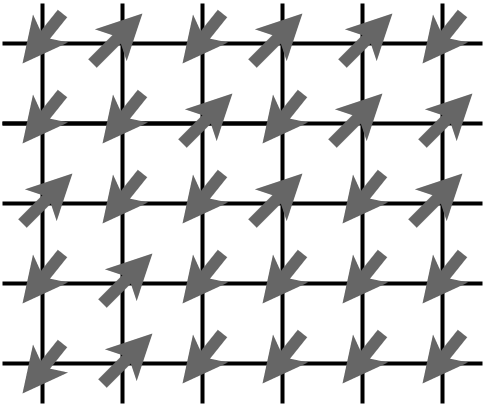
\includegraphics[keepaspectratio, scale=0.3]{./doc/img/KW_duality.png}
				\subcaption{2次元Ising模型.格子「点」上にスピンが並んでいる.}
		\end{minipage}
		\begin{minipage}[t]{0.32\linewidth}
				\centering
				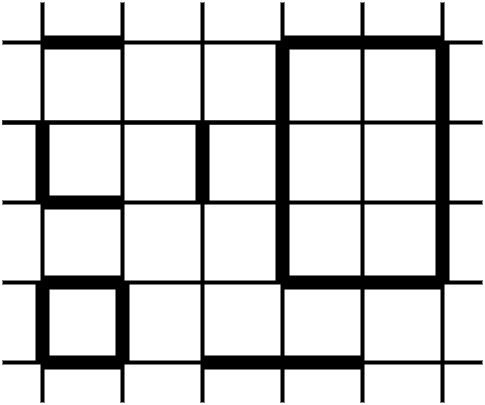
\includegraphics[keepaspectratio, scale=0.3]{./doc/img/KW_duality-Page-2.drawio.png}
				\subcaption{各辺に$0, 1$を割り当てる(Eq. \eqref{KW01}).この図においては太線が1と思うことにする.}
		\end{minipage}
		\begin{minipage}[t]{0.32\linewidth}
				\centering
				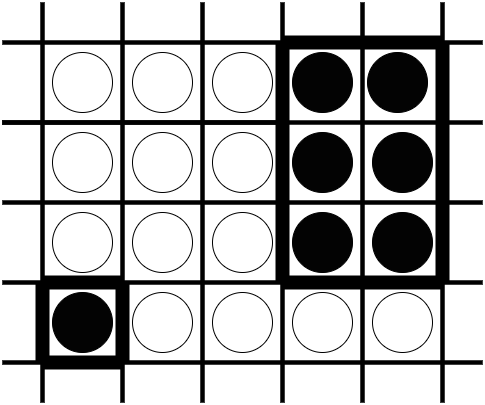
\includegraphics[keepaspectratio, scale=0.3]{./doc/img/KW_duality-Page-3.drawio.png}
				\subcaption{寄与があるのは太い閉曲線のみ(Eq. \eqref{close_KW}).閉曲線の中と外という二つの状態があるので,格子の「中」に黒丸と白丸の新しいスピンがあると思える(Eq. \eqref{new_spin}).}
		\end{minipage}
		\caption{Kramers--Wanneir双対性の分配関数の操作の概略.}
		\label{fig:KW_load}
\end{figure}


	ひたすら分配関数を書き換えてゆく.Figure \ref{fig:KW_load}に操作の手順をまとめた.まず,
	\begin{equation}
			e^{K\sigma_i \sigma_j} = \cosh K \sum_{t\in\qty{0, 1}}\qty(\sigma_i \sigma_j \tanh K)^t
	\end{equation}
	と書き換える.よくわからないが,正しいことは少し計算すればわかる.これは各スピンのペアに対して定まり,ペアに関して積をとることはそれらを結ぶ辺について積をとることと同じであることに注意すると,次のように書き換えることができる.

	\begin{align}
			Z(K) &= \sum_{\sigma} e^{K\sum_{\langle i, j\rangle}\sigma_i\sigma_j}\\
				 &= \sum_{\sigma} \prod_{\langle i, j \rangle}e^{K\sigma_i \sigma_j}\\
				 &= \qty(\cosh K)^{2N} \sum_{\sigma}\sum_{\qty{t}}\prod_{\text{辺}}\qty(\sigma_i \sigma_j\tanh K)^t\label{KW01}
	\end{align}
	$\sum_{\qty{t}}$は,各辺に$0, 1$を割り当てるすべての配位に関する和で,$\prod_{\text{辺}}$は一つ選んだ配位に関して積をとる操作である.
	この積について,$t=0$が与えれられた辺は$1$で寄与する.
	$t = 1$が与えられた配位について考える.先に$\sigma$についての和をとることを考える.これは有限和なので,文句なしに可能である.
	このとき,各$\sigma_i$でくくると,$n\in\Z$とすると
	\begin{align}
			\sum _{\sigma_i = \pm1}\sigma_i^{2n-1} &= 0,\\
			\sum_{\sigma_i = \pm1} \sigma_i^{2n} &= 2
	\end{align}
	であるので,$t=1$が偶数個集まる点からは$2\tanh K$で寄与する.
	模型に対応付けると,$t = 1$の線が一つだけ集まることは線の端があることに対応して,一つでもこれがあると積はゼロになるので,閉曲線になっているところだけが積に寄与することになる.

	結局,分配関数は
	\begin{align}
			Z(K) &= \qty(\cosh K)^{2N}\sum_{\qty{\text{閉曲線}}}\qty(2\tanh K)^{\text{閉曲線の長さ}}\\
				 &= \qty(2\cosh K)^{2N}\sum_{\qty{\text{閉曲線}}}\qty(2\tanh K)^{\text{閉曲線の長さ}}\label{close_KW}
	\end{align}
	となる.ここで,格子には閉曲線の中と外という二つの状態ができる.これをスピンの上下に対応させることを考える.このスピン配位を$\mu$と書くことにする.

	今,閉曲線に関して和を取っているが,これはスピンの配位$\mu$に関して和を取っているとおもってもよい.
	また,閉曲線周りでは隣接するスピンは逆向きで,$\mu_i \mu_j = -1$になるので,$(1-\mu_i\mu_j)/2$で隣接する$i, j$について和をとると閉曲線で$1$, そうでない場所で$0$と区別ができる.
	さて,分配関数は
	\begin{align}
			Z(K) &= \qty(2\cosh K)^{2N} \sum_{\qty{\mu}} \prod_{\text{辺}}(\tanh K)^{(1-\mu_i\mu_j)/2}\\ 
			&= \qty(2\cosh K)^{2N}(\tanh K)^N\sum_{\mu}\prod_{\langle i, j \rangle}\qty(\tanh K)^{\mu_i\mu_j/2}\\
			&= (\sinh 2K)^{N/2}Z(K')\label{new_spin}
	\end{align}
	と変形できる.ここで,$e^{K'} = \tanh^{-1/2} K$とおいた.つまり,パラメータ$K$の二次元イジングモデルは$K'$の二次元イジングモデルと関係していることがわかる.この関係をKramers--Wanneir双対性\cite{PhysRev.60.252}という.

	さて,この変換を二回行うと
	\begin{equation}
			Z(K) = (\sinh K \sinh K')^NZ(K)
	\end{equation}
	となるので,$\sinh 2K \sinh 2K' = 1$でないといけない.$\sinh$は単調関数なので,変なことが起こるとすれば$K = K'$と予想できる.
	これを解くと,
	\begin{equation}
			K_{\text{c}} = \frac{1}{2}\log(1 + \sqrt{2}) \sim 0.4407 \label{Tc_2d-Ising}
	\end{equation}
	となる.この解は正しい臨界温度を与えることが知られている.



